\section{State-space representation}

% Open loop model description
\subsection{Open loop model description}
Input vector $U$ and state vector $X$ are given by :
$$
U = \begin{pmatrix}
    F_1 \\
    u
\end{pmatrix}
\hspace{3cm}
X = \begin{pmatrix}
    d_1 \\
    \dot d_1 \\
    d_2 \\ 
    \dot d_2 \\
\end{pmatrix}
$$

\subsubsection{Inputs}
\begin{itemize}
    \item $F_1(t)$, the force of the wind (uncontrollable), approximately between \num{1000} and \SI{2000}{\kilo\newton}.
    \item $u(t)$, the force applied on the mass damper (controllable), approximately between \num{1000} and \SI{2000}{\kilo\newton}.
\end{itemize}
Our sensor is a measurement of the horizontal position of the top of the building relatively to the vertical position $d_1 = 0$.\par
Our actuator provides a force on the mass of the dampener, sets it in motion.

\subsubsection{Outputs}
$y = d_1(t)$ the relative position of the building with respect to the vertical position.

\subsubsection{States}
\begin{itemize}
    \item $x_1 = d_1$, as described above, ranging from a few millimeters to a few meters.
    \item $x_2 = \dot d_1$, the speed of the building, ranging from about \num{0.1} to \SI{5}{\meter\per\second}.
    \item $x_3 = d_2$, the relative displacement of the mass damper, ranging from a few millimeters to a few meters.
    \item $x_4 = \dot d_2$, the speed of the mass damper, ranging from about \num{0.1} to \SI{5}{\meter\per\second}.
\end{itemize}

\subsubsection{Output law}
The output is one of the states : $y = x_1$.

\subsubsection{Input law}
The input law is given by \cite{sciencedirect_amd} :
$$
\begin{cases}
    m_{1}\ddot{d}_{1} + c_{1}\dot{d}_{1} + k_{1}d_{1} = c_{2}\dot{z} + k_{2}z + F_{1}(t) - u(t)\\
    m_{2}\ddot{z} + c_{2}\dot{z} + k_{2}z = -m_{2}\ddot{d}_{1} + u(t)
\end{cases}
$$
with $z = d_2 - d_1$.

% State-space model
\subsection{State-space model}
The system is \textbf{linear}. We can easily derive the ABCD matrices.
$$
A = \begin{pmatrix}
    0 & 1 & 0 & 0 \\
    \frac{-k_1-k_2}{m_1} & \frac{-c_2-c_1}{m_1} & \frac{k_2}{m_1} & \frac{c_2}{m_1} \\
    0 & 0 & 0 & 1 \\ 
    \frac{k_2}{m_2} & \frac{c_2}{m_2} & \frac{-k_2}{m_2} & \frac{-c_2}{m_2}\\
\end{pmatrix}
\quad
B = \begin{pmatrix}
    0 & 0\\
    \frac{1}{m_1} & -\frac{1}{m_1}\\
    0 & 0\\
    0 & \frac{1}{m_2}\\
\end{pmatrix}
$$
$$
C = \begin{pmatrix}
    1 & 0 & 0 & 0\\
\end{pmatrix}
\quad
D = \begin{pmatrix}
    0 & 0\\
\end{pmatrix}
$$

% Constraints, limitations and numerical choice of parameter values
\subsection{Constraints, limitations and numerical choice of parameter values}
To model and study the system, we defined a series of constraints, assumptions and limitations, presented in table \ref{tab:constraints_assumptions_limitations}.\par
\begin{table}[H]
    \centering
    \begin{tabular}{|l|c|}
        \hline
        \multirow{2}{*}{{\bf Building}} & height of \SI{200}{\meter}, width of \SI{30}{\meter}\\ & movement along a single axis (horizontal)\\\hline
        {\bf Mass} & no friction between $m_1$ and $m_2$\\ \hline
    \end{tabular}
    \caption{Constraints, assumptions and limitations of the system.}
    \label{tab:constraints_assumptions_limitations}
\end{table}
To simulate the system (without control mechanism), we choose a series of numerical values, presented in table \ref{tab:numerical_values}\footnote{We would like to thank Professor Denoël for discussing these values with us.}.
\begin{table}[H]
    \centering
    \begin{tabular}{|l|c|c|}
        \hline
        {\bf Mass} & $m_1 = \SI{1e7}{\kilogram}$ & $m_2 = \SI{3e3}{\kilogram}$\\ \hline
        {\bf Spring} & $k_1 \approx \SI{4e8}{\newton/\meter}$ & $k_2 = \SI{e5}{\newton/\meter}$\\ \hline
        {\bf Damper} & $c_1 \approx \SI{1.3e6}{\newton\second/\meter}$ & $c_2 = \SI{e4}{\newton\second/\meter}$\\ \hline
        {\bf Wind} & \multicolumn{2}{c|}{$F_{max} = \SI{810000}{\newton}$}\\ \hline
    \end{tabular}
    \caption{Numerical values of the system}
    \label{tab:numerical_values}
\end{table}
For the strength of the wind, we considered 2 cases (in newton) :
\begin{align*}
    F_1 &= F_{max}\quad\forall t & \text{Constant wind force}\\
    F_1(t) &= F_{max}\sin(2\pi t) & \text{Sinusoidal wind force}
\end{align*}
The stiffness and viscosity values for the building were obtained using the formulas :
\begin{align*}
    k_1 &= (2\pi f)^2m_1\\
    c_1 &= 2m_1(2\pi f)0.01
\end{align*}
where $f = \SI{1}{\hertz}$ is the natural frequency associated with the mass of the building.\par
The maximum wind force, on the other hand, was approximated by
\begin{equation*}
    F_{max} = \frac{1}{2}\rho v^2A
\end{equation*}
with
\begin{itemize}
    \item $\rho \approx \SI{1.2}{\kilogram/\meter\cubed}$, the air density;
    \item $v = \SI{15}{\meter/\second}$, the wind speed;
    \item $A = 200\times 30 = \SI{6000}{\meter\squared}$, the area of one side of the building.
\end{itemize}

% Stability and eigenvalues
\subsection{Stability and eigenvalues}
To study the stability of the system, we compute the eigenvalues of the dynamic matrix $A$ thanks to Matlab function (\texttt{eig}) :
\begin{align*}
    \lambda_1 &= \num{-0.0645 + 6.2824i}\\
    \lambda_2 &= \num{-0.0645 - 6.2824i}\\
    \lambda_3 &= \num{-1.6655 + 5.5285i}\\
    \lambda_4 &= \num{-1.6655 - 5.5285i}
\end{align*}
The system is stable if the real parts of the eigenvalue are all negative. In our case, the system is stable.

% Open loop system simulations
\subsection{Open loop system simulations}
\begin{figure}[H]
    \centering
    \begin{subfigure}{0.495\textwidth}
        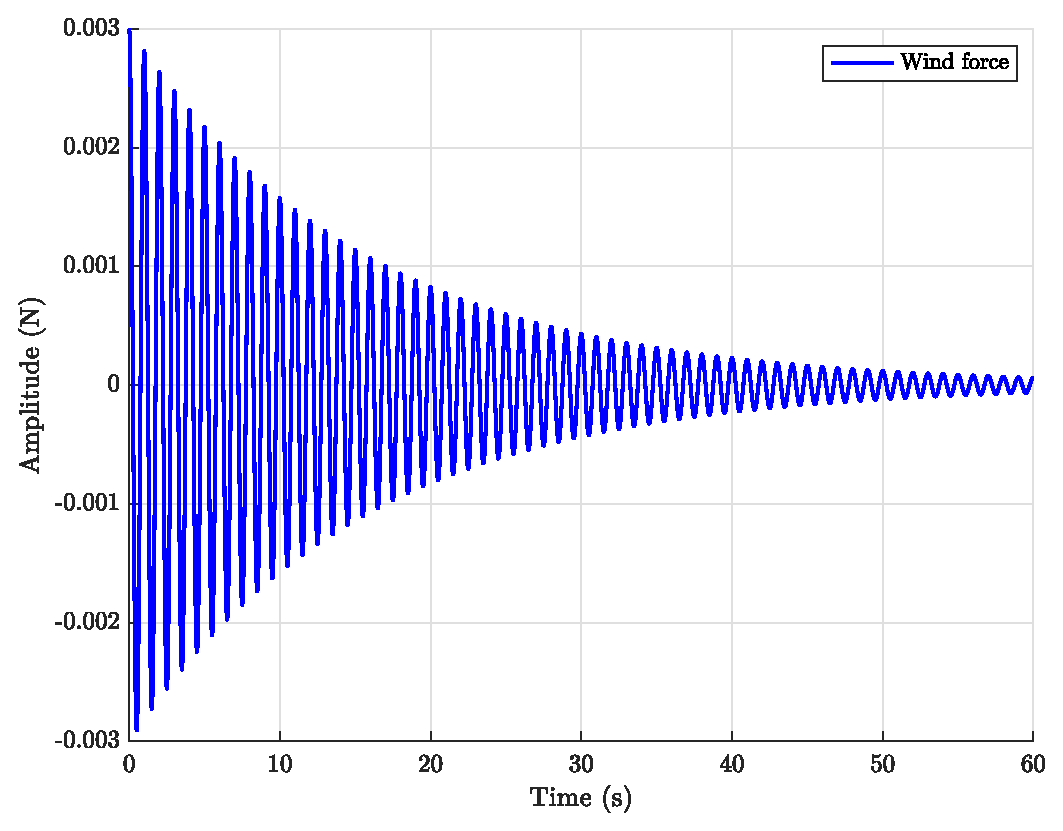
\includegraphics[width=\textwidth]{resources/eps/initial-condition.eps}
        \caption{Initial conditions}
        \label{fig:q4.initial}
    \end{subfigure}
    \begin{subfigure}{0.495\textwidth}
        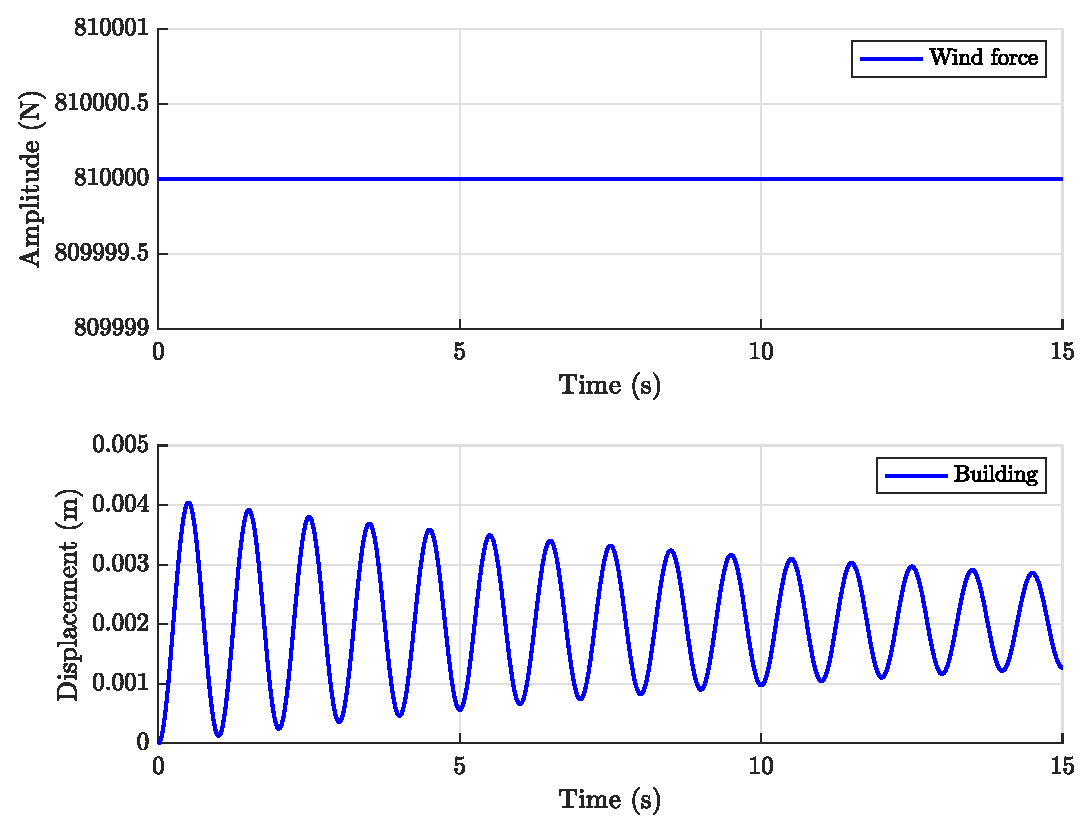
\includegraphics[width=\textwidth]{resources/eps/constant-wind.eps}
        \caption{Constant wind force}
        \label{fig:q4.constant}
    \end{subfigure}
    \begin{subfigure}{0.495\textwidth}
        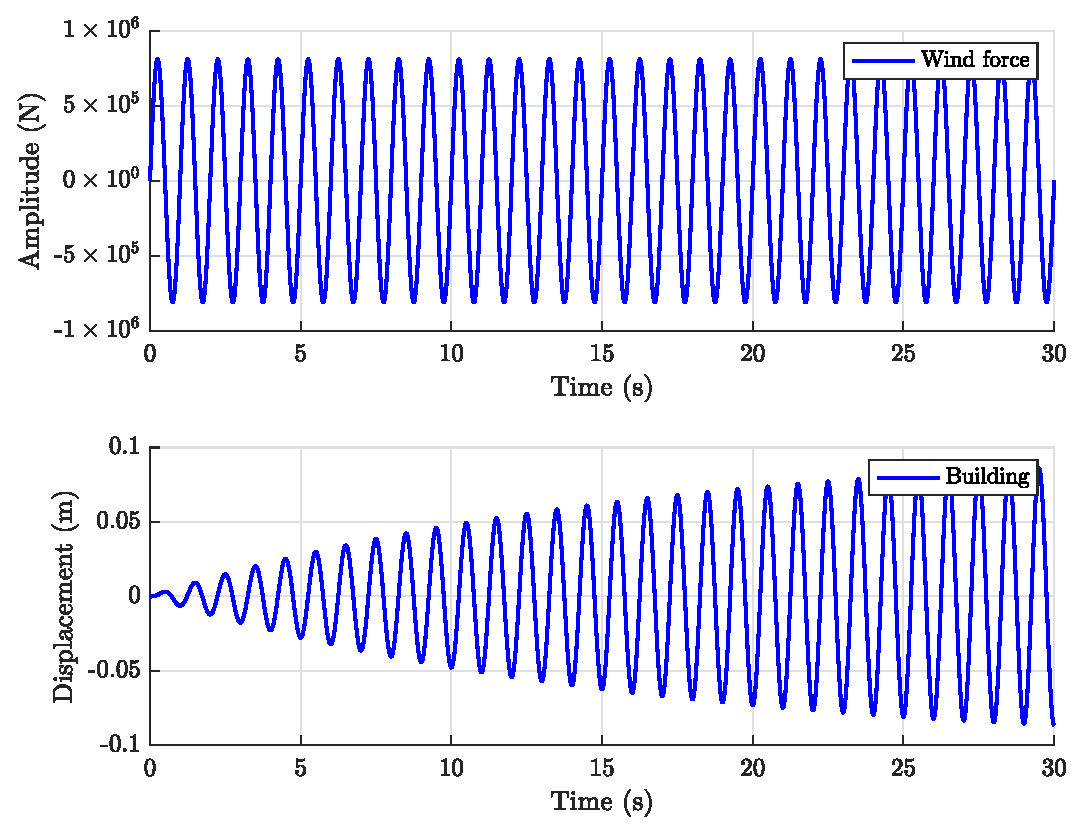
\includegraphics[width=\textwidth]{resources/eps/sinusoidal-wind.eps}
        \caption{Sinusoidal wind force}
    \end{subfigure}
    \begin{subfigure}{0.495\textwidth}
        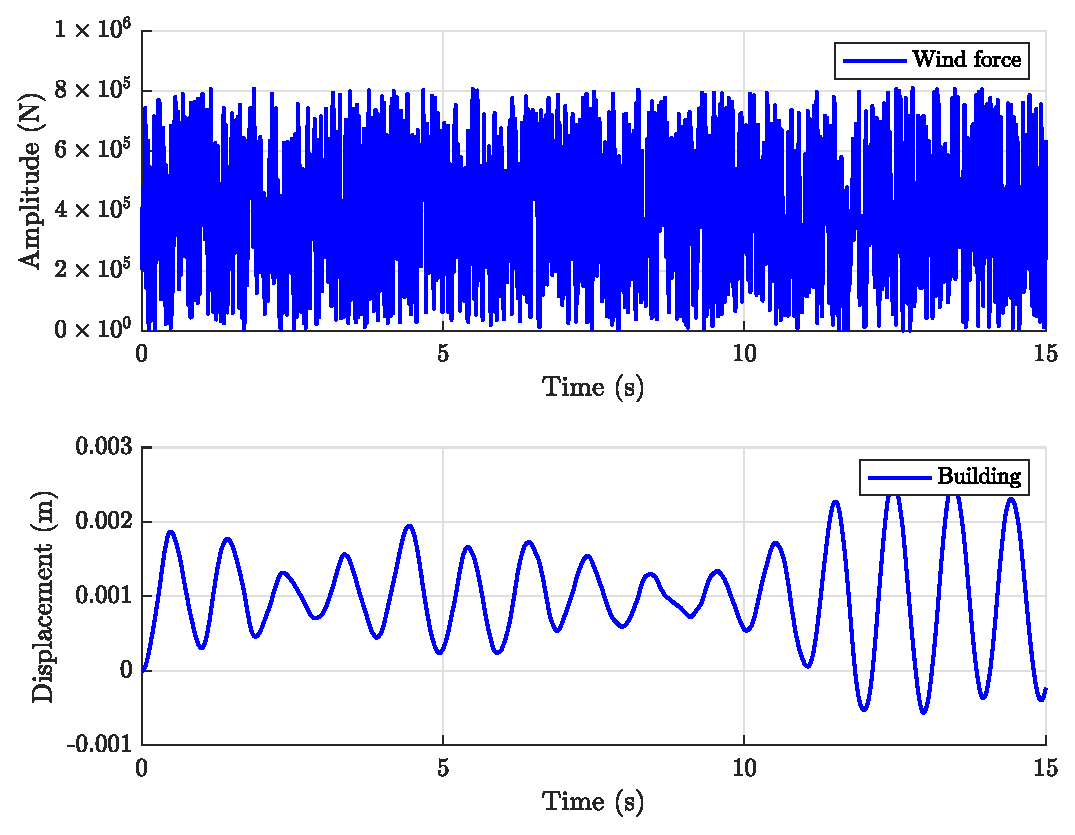
\includegraphics[width=\textwidth]{resources/eps/random-wind.eps}
        \caption{Random wind force}
    \end{subfigure}
    \noskipcaption{Simulation results}
\end{figure}
The first simulation (figure \ref{fig:q4.initial}) is a response of our system to initial conditions : the initial displacement of the building is defined at \SI{0.5}{\meter}. We observe that the building oscillates and tends to regain its reference position.\par
The other simulations are responses of our system to an input (the wind).\par
In the case of a constant force (figure \ref{fig:q4.constant}), the building oscillates at the beginning and then tends to stabilize (at a position different from its reference).\par
In cases of sinusoidal and random forces, the building oscillates and follows approximately the wind movement.

% Observability
\subsection{Observability}
To determine whether or not the system is observable, we compute the observability matrix thanks to Matlab function (\texttt{obsv}).\par
The matrix is full rank (verified with Matlab), the system is thus fully observable.\par
As seen on the matrix C, we need one sensor. According to the place of the non zero value, this sensor has to measure the $x_1$ state, namely the horizontal position of the top of the building $d_1$. This state is indeed the objective of the active mass damper and has thus to be observed.

% Controllability
\subsection{Controllability}
To determine whether or not the system is controllable, we compute the controllable matrix thanks to Matlab function (\texttt{ctrb}). In order not to take into account the uncontrollable input (wind), only the second column of the B matrix was kept for the calculation.\par
The matrix is full rank (verified with Matlab), the system is thus fully controllable.\par
As seen on matrix B, we need only one actuator. The first column of the $B$ matrix represents the wind, while the second one concerns the damper. This latter is indeed the only controllable input and contains two non-zero elements. As a result, only one actuator is needed, and acts on two states, the speed of the building and the speed of the damper, as they take place on $x_2$ and $x_4$.
